% Dots

This domain is a perception example.
The true numbers of points are, respectively, 320, 310, 300, 290 and 280.
It is much clearer that there are more points in the first panel than in the fifth, than that there are more points in the first than in the second.
The difference in the number of points is an obvious similarity measure here that might be expected to lead to similarity effects.
{}
\begin{tcolorbox}
Which one of the following boxes do you think has the greatest number of points?

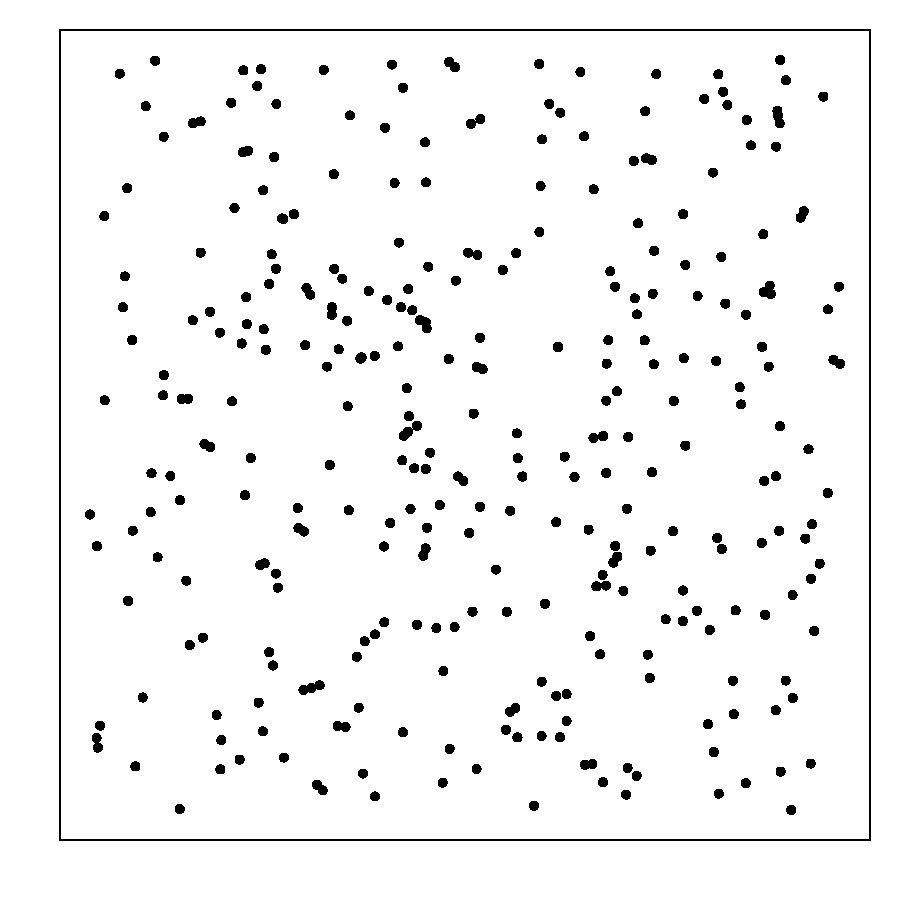
\includegraphics[height=3cm]{Scatterplots1.pdf}
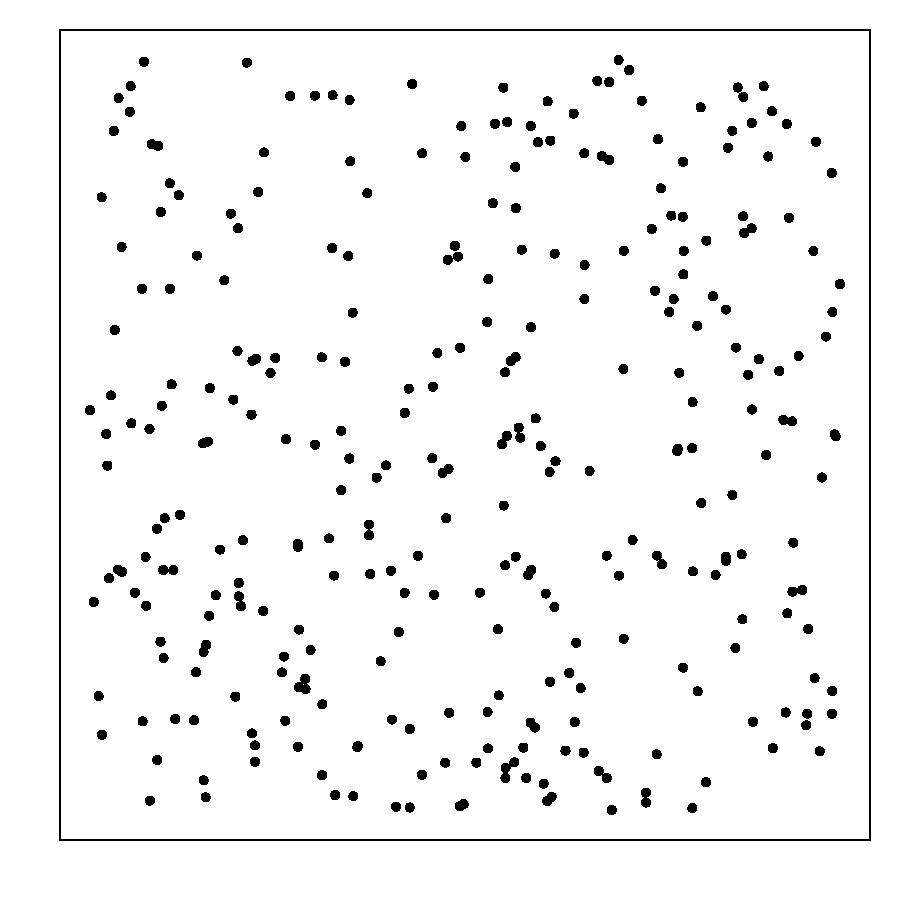
\includegraphics[height=3cm]{Scatterplots2.pdf}
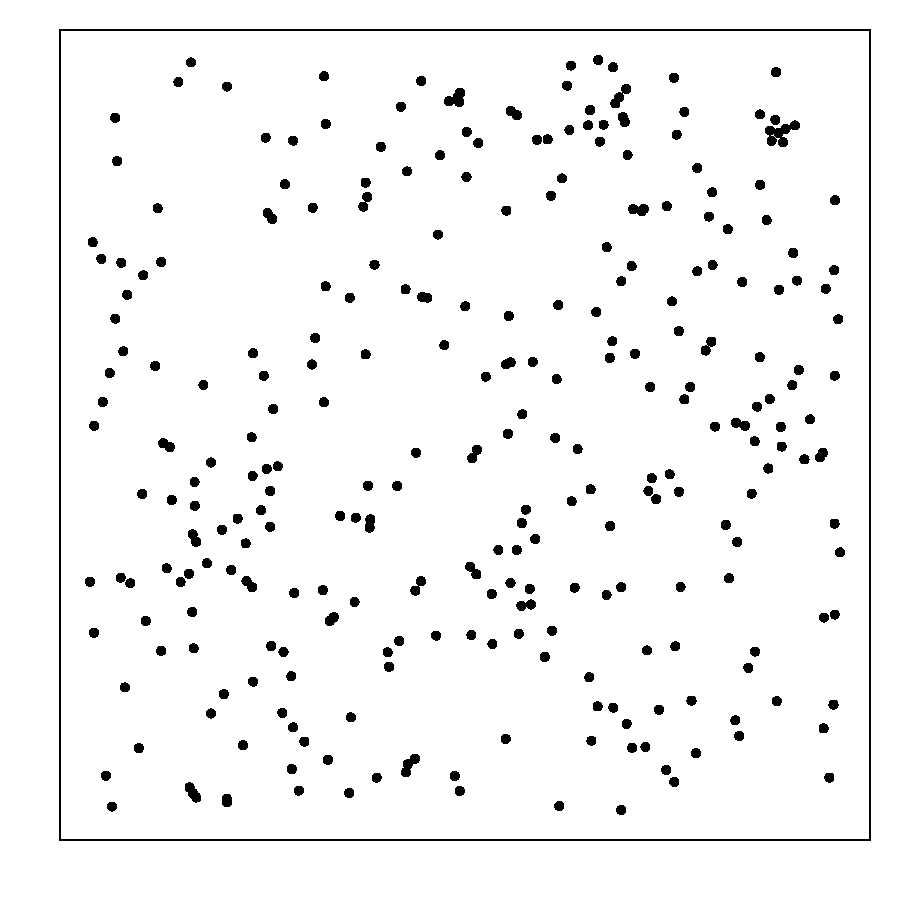
\includegraphics[height=3cm]{Scatterplots3.pdf}
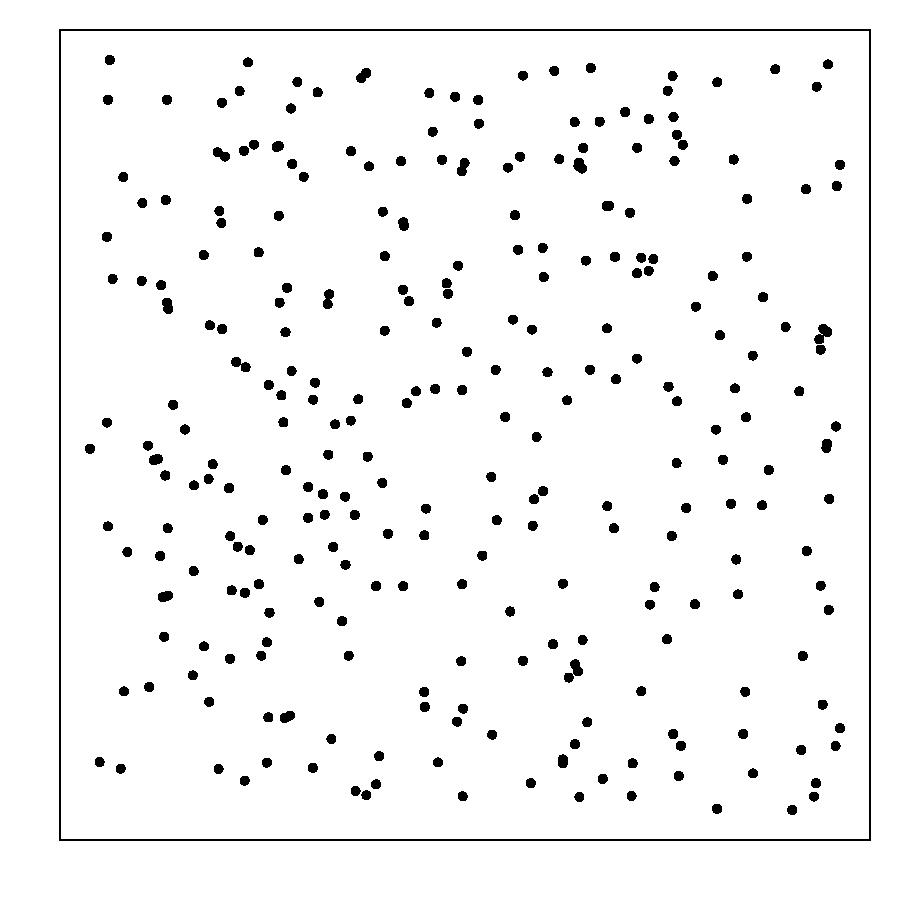
\includegraphics[height=3cm]{Scatterplots4.pdf}
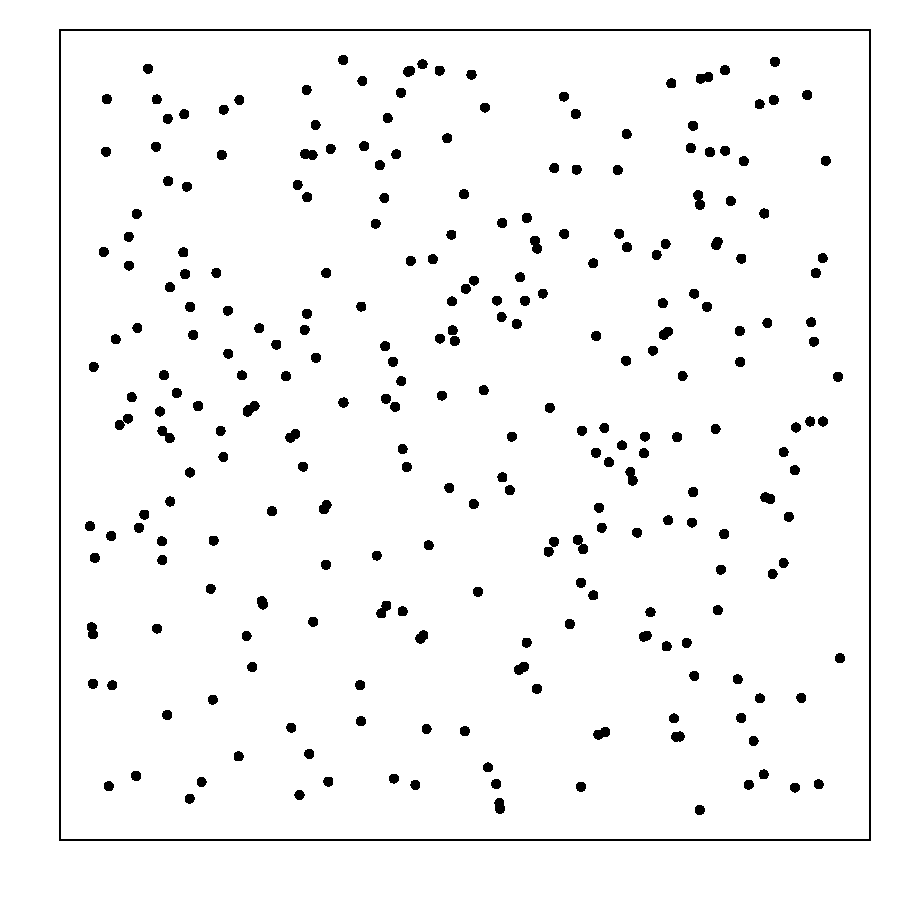
\includegraphics[height=3cm]{Scatterplots5.pdf}
\end{tcolorbox}
